\documentclass[11pt,a4paper]{article}
\usepackage[T1]{fontenc}
\usepackage[utf8]{inputenc}
\usepackage{lmodern}
\usepackage[margin=2.2cm]{geometry}
\usepackage{amsmath,amssymb}
\usepackage{booktabs,tabularx,array}
\usepackage{graphicx}
\usepackage{xcolor}
\usepackage{caption}
\usepackage{float}
\usepackage[colorlinks=true,linkcolor=blue!45!black,urlcolor=blue!45!black,citecolor=blue!45!black]{hyperref}
\graphicspath{{figures/}}
\newcommand{\code}[1]{\texttt{\detokenize{#1}}}
\newcommand{\keybox}[1]{\par\smallskip\noindent\fcolorbox{black!35}{black!4}{\parbox{\dimexpr\linewidth-2\fboxsep-2\fboxrule}{#1}}\par\smallskip}
\newcolumntype{L}{>{\raggedright\arraybackslash}X}
\setlength{\parskip}{4pt}
\setlength{\parindent}{0pt}
\setlength{\emergencystretch}{3em}
\captionsetup{font=small,labelfont=bf,skip=4pt}
\DeclareMathOperator*{\argmax}{arg\,max}
\newcommand{\E}{\mathbb{E}}
\newcommand{\1}{\mathbf{1}}

\title{\vspace{-1.2cm}The SPO tree under regime-dependent volatility: experiments and results\\[2pt]\large A second synthetic market: the price volatility also follows a threshold on the feature}
\author{}
\date{23 September 2026}

\begin{document}
\maketitle
\vspace{-0.6cm}

\keybox{\textbf{In short.} The planted-threshold experiments (\code{experiments_planted_threshold.tex}) use a market whose drift follows a threshold on one feature $x$ while the volatility stays constant. Here the volatility follows a threshold too: 1\% a day in the \emph{stress} regime, 0.5\% a day in the \emph{calm} one. Two questions. Does the tree still find the drift threshold when the noise is not the same on both sides of it? And when the volatility threshold sits elsewhere than the drift threshold, so that the right position between the two is a \emph{smaller} one rather than a different sign, does the tree find that second boundary? The second question only has content when the risk aversion is large enough for the position to depend on the variance, so every setting is run at $\lambda=1$ and $\lambda=10$.

\textbf{Results} (Section~\ref{sec:results}, 2{,}240 fitted trees).
\begin{itemize}\setlength{\itemsep}{1pt}
\item \textbf{The drift threshold is found, and found better, when the bad regime is the noisy one.} With the volatility threshold at $d$, the first split is within $0.25$ of $d$ in 95\% of the datasets at weekly decisions (84\% with constant volatility) and the threshold is found in 88\% of the monthly datasets (72\%): the good regime's returns are cleaner, and they pin the threshold. Every Sharpe ratio nearly doubles, the ideal rule's as much as the tree's, and the tree keeps 83 to 86\% of the ideal gain.
\item \textbf{The volatility boundary is not found.} With the volatility threshold at $d+1$ and $\lambda=10$, only 8 to 12\% of the trees keep a split near $x=1$, and their position in the calm regime (0.52 of the asset) follows the ideal rule on the same information (0.58), not the clairvoyant one (0.96). The reason is structural: the regret that trains the tree is computed with the same lagged covariance estimate as the optimizer uses, so a boundary that exists only in the true variance is invisible to the loss.
\item \textbf{A shorter covariance window does not fix it.} With 20 days instead of 180 the estimate follows the regime, and the tree does size up in the calm regime (0.69 to 0.75), but the estimate's noise costs more than the regime tracking gains: the ideal rule itself falls from 1.16 to 1.10 at weekly decisions.
\item Knowing the current variance is worth about 0.1 of annual Sharpe at the fast rates when the volatility boundary sits inside the good regime (ideal rule 1.16, with the true variance 1.23), and nothing when the volatility and drift regimes coincide.
\end{itemize}
}

\section{The model}\label{sec:model}
The feature is the daily Ornstein--Uhlenbeck process of the planted-threshold report, $x_{t+1}=m+e^{-k}(x_t-m)+\eta_t$ with $\eta_t\sim\mathcal N(0,s^2(1-e^{-2k}))$, and the price is a geometric random walk whose drift \emph{and} volatility follow $x$ (\code{synthetic_market.signal_process} with \code{up_volatility_ratio} and \code{volatility_threshold}):
\begin{equation}\label{eq:price}
\log\frac{S_{t+1}}{S_t}=\mu_t-\tfrac12\sigma_t^2+\sigma_t\varepsilon_t,\qquad
\mu_t=\begin{cases}+\mu & x_t\ge d\\ -\mu & x_t<d\end{cases},\qquad
\sigma_t=\begin{cases}\rho\,\sigma & x_t\ge d_\sigma\\ \sigma & x_t<d_\sigma\end{cases},
\end{equation}
with $\sigma=1\%$ a day, $\rho=0.5$ (calm regime at half the volatility) and $\mu=e\sigma$ as before, $e$ the edge. With $d_\sigma=d$ the stress regime is exactly the bad regime, the usual picture of markets; with $d_\sigma=d+1$ (one standard deviation of $x$ above the drift threshold) the good regime is split into a stressed part, $d\le x<d_\sigma$, and a calm part, $x\ge d_\sigma$.

\textbf{What a correct tree should do.} The expected simple return over a holding period of $h$ days given $x$ now, $g_h(x)=\E[e^{\mu B_h}\mid x_0=x]-1$ with $B_h$ the days spent above $d$ minus the days below, does not depend on the volatility: the price noise averages out. So the drift threshold is where it was, at $d=m$. The volatility enters through the position. For the asset against cash the optimizer gives
\begin{equation}\label{eq:w}
w=\frac{g_h(x)\mp f}{2\lambda\sigma_h^2}\ \text{clipped to }[0,1],
\end{equation}
where $\sigma_h^2$ is the variance of the return over the holding period as the optimizer knows it. In the stress regime $2\lambda\sigma_h^2$ is $0.1\%$ at weekly decisions with $\lambda=1$ and $1\%$ with $\lambda=10$; in the calm regime a quarter of that. Against expected returns of up to $0.5\%$ this means:
\begin{itemize}\setlength{\itemsep}{1pt}
\item at $\lambda=1$ the position is all or nothing in both regimes, and the volatility threshold is invisible to the decision; the volatility only changes how noisy the training decisions are;
\item at $\lambda=10$ the ideal position is about one half in the stressed good regime and one in the calm good regime: with $d_\sigma=d+1$ the decision has a second boundary at $x=1$, of size rather than of sign, and a tree that wants it must add a second split there.
\end{itemize}
Two versions of the ideal rule are replayed. The \emph{ideal rule} feeds the optimizer with the true $g_h(x)$ and the same covariance as the tree, $\Sigma_t=h\,\widehat{\mathrm{Var}}(\text{last }H\text{ daily returns})$, which lags the regime; the \emph{ideal rule with the true variance} uses the regime's own variance on the decision day, $h\sigma_t^2$, which no estimator has. The difference between the two is the price of not knowing the current volatility.

\begin{table}[H]
\centering\small
\begin{tabularx}{\linewidth}{@{}l L@{}}
\toprule
Setting & What it is\\
\midrule
constant volatility, $\lambda=1$ and $10$ & the market of the planted-threshold report ($\rho=1$): the reference\\
volatility threshold at $d$, $\lambda=1$ and $10$ & $d_\sigma=d=0$: the bad regime is the stress regime\\
volatility threshold at $d+1$, $\lambda=1$ and $10$ & $d_\sigma=1$: the good regime is stressed below $x=1$ and calm above\\
volatility threshold at $d+1$, $\lambda=10$, 20-day covariance & the same, with $\Sigma_t$ estimated on the last 20 days instead of 180, so that it can follow the regime\\
\bottomrule
\end{tabularx}
\caption{The seven settings. Everything else is the base case of the planted-threshold report: $k=0.02$ (half-life 35 days), $x$ standardized, $d=0$, fee 3 bp, tree of depth 2 with at least 20 decisions per leaf, pruning on the last quarter of the training decisions.}
\label{tab:settings}
\end{table}

\section{Protocol}\label{sec:protocol}
\textbf{Pipeline used.} P3b of \code{model_history.md} with every split-search option off, identical to P2 (plain splits, every threshold screened, depth 2, 20 decisions per leaf, pruning on the last quarter); $\lambda=1$ or $10$ and a covariance window of 180 or 20 days as listed in Table~\ref{tab:settings}; market M2' with the volatility threshold.

The protocol is that of the planted-threshold report, Section~8: decisions every 2, 5, 10 and 21 days, edges 0.05 and 0.10 (regime drift $\pm13\%$ and $\pm25\%$ a year), 15 years of training and 5 years of test, 40 independent datasets per cell, the tree replayed on the test years against the two ideal rules, the rule at $d$ and always holding the asset. Measurements: whether the first split is on $x$ and where; whether a second-level split lands within $0.25$ of the volatility threshold; the mean position taken on the test decisions by bin of $x$; the annualized test Sharpe ratio; the share of the ideal rule's gain captured.

\section{Results}\label{sec:results}
\begin{figure}[H]
\centering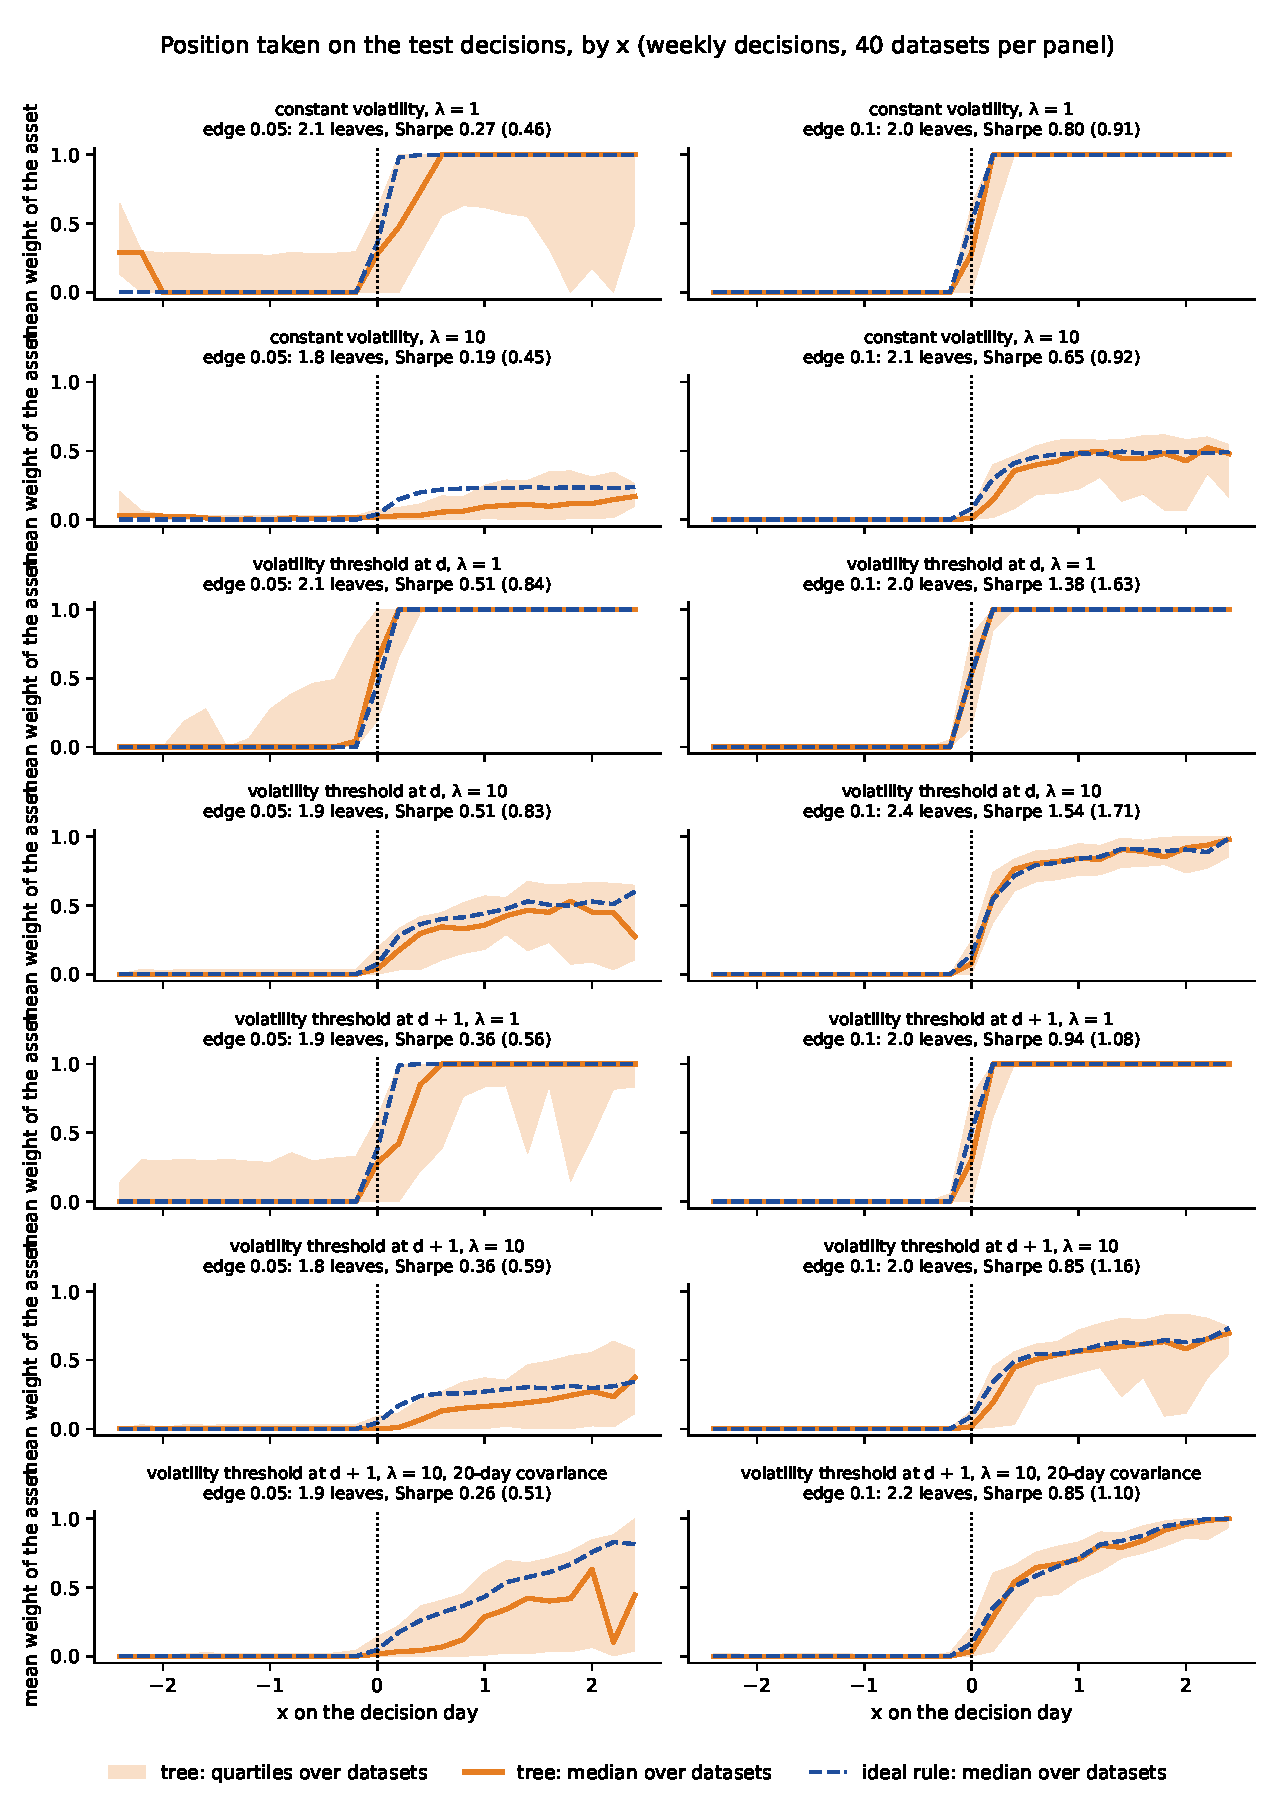
\includegraphics[width=0.85\linewidth]{regime_volatility_positions}
\caption{Weekly decisions: the weight of the asset taken on the test decisions, by $x$ on the decision day, one row per setting; \emph{left:} edge 0.05, \emph{right:} edge 0.10. Orange: the tree (median over the 40 datasets, quartiles as a band); dashed blue: the ideal rule on the same information as the tree. Panel titles: mean number of leaves, annualized test Sharpe ratio of the tree (ideal rule in brackets).}
\label{fig:positions}
\end{figure}
\begin{figure}[H]
\centering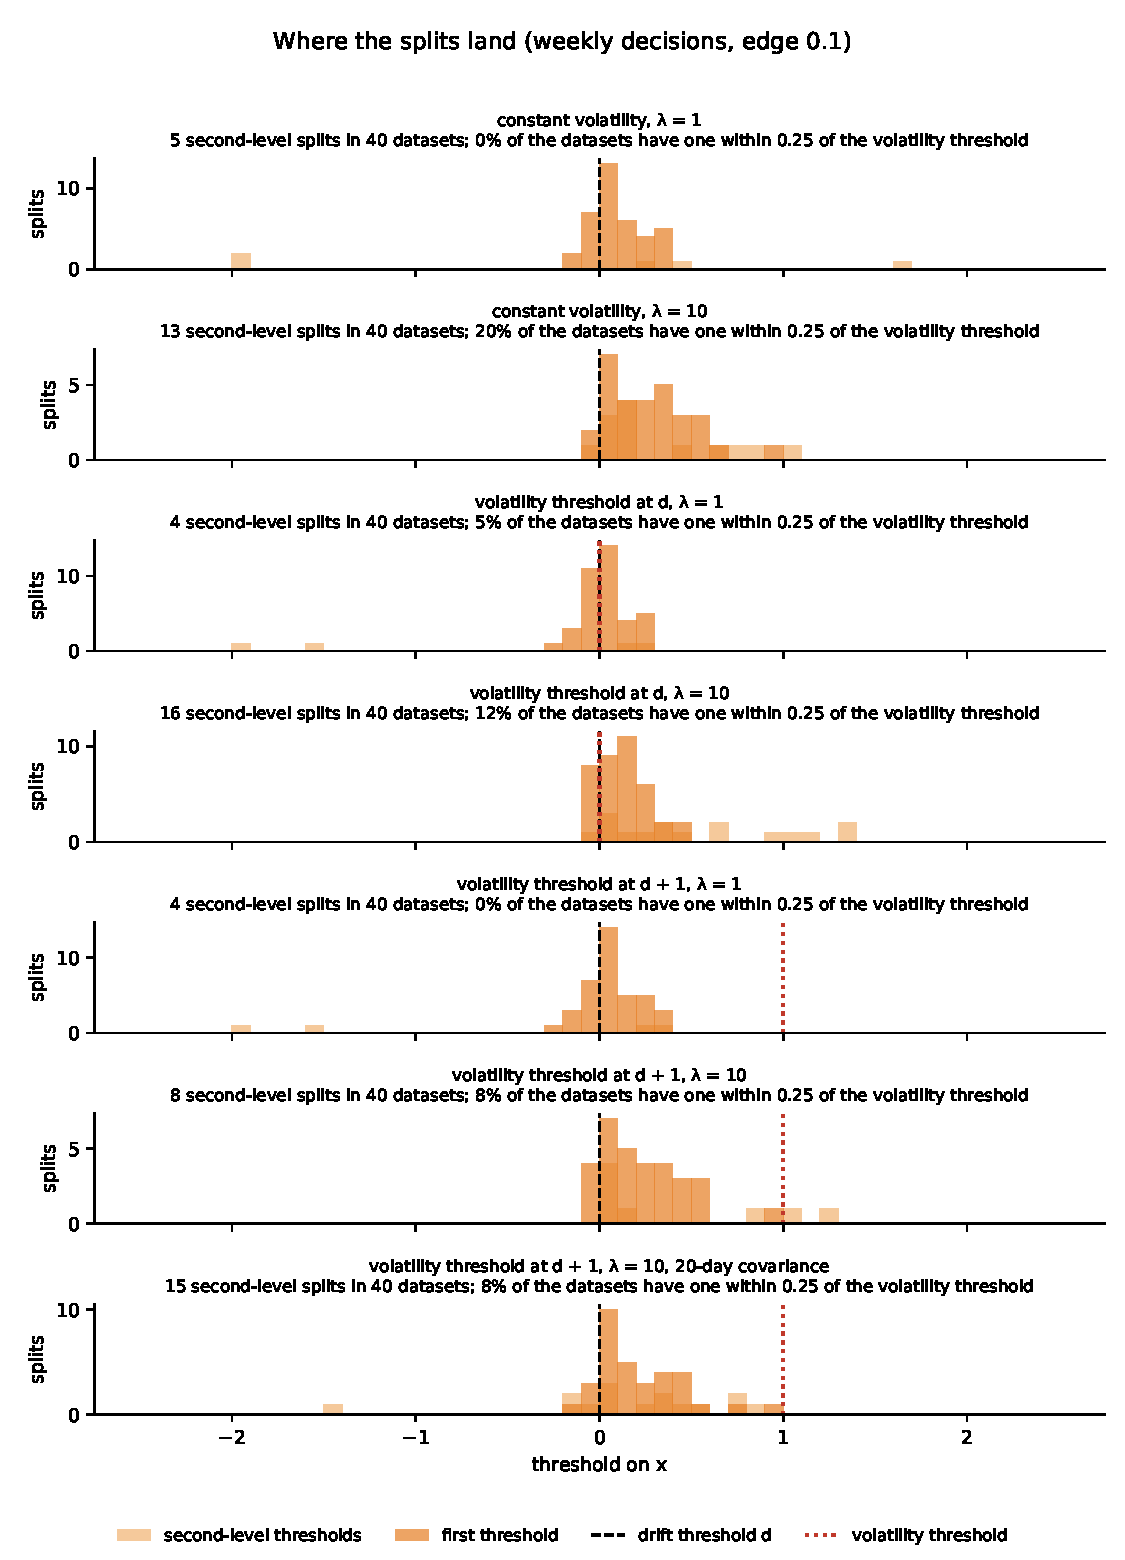
\includegraphics[width=0.9\linewidth]{regime_volatility_splits}
\caption{Weekly decisions, edge 0.10: every threshold kept, first splits in orange and second-level splits in light orange, with the drift threshold (dashed) and the volatility threshold (dotted red). The second-level splits do not gather at the volatility threshold.}
\label{fig:splits}
\end{figure}
\begin{figure}[H]
\centering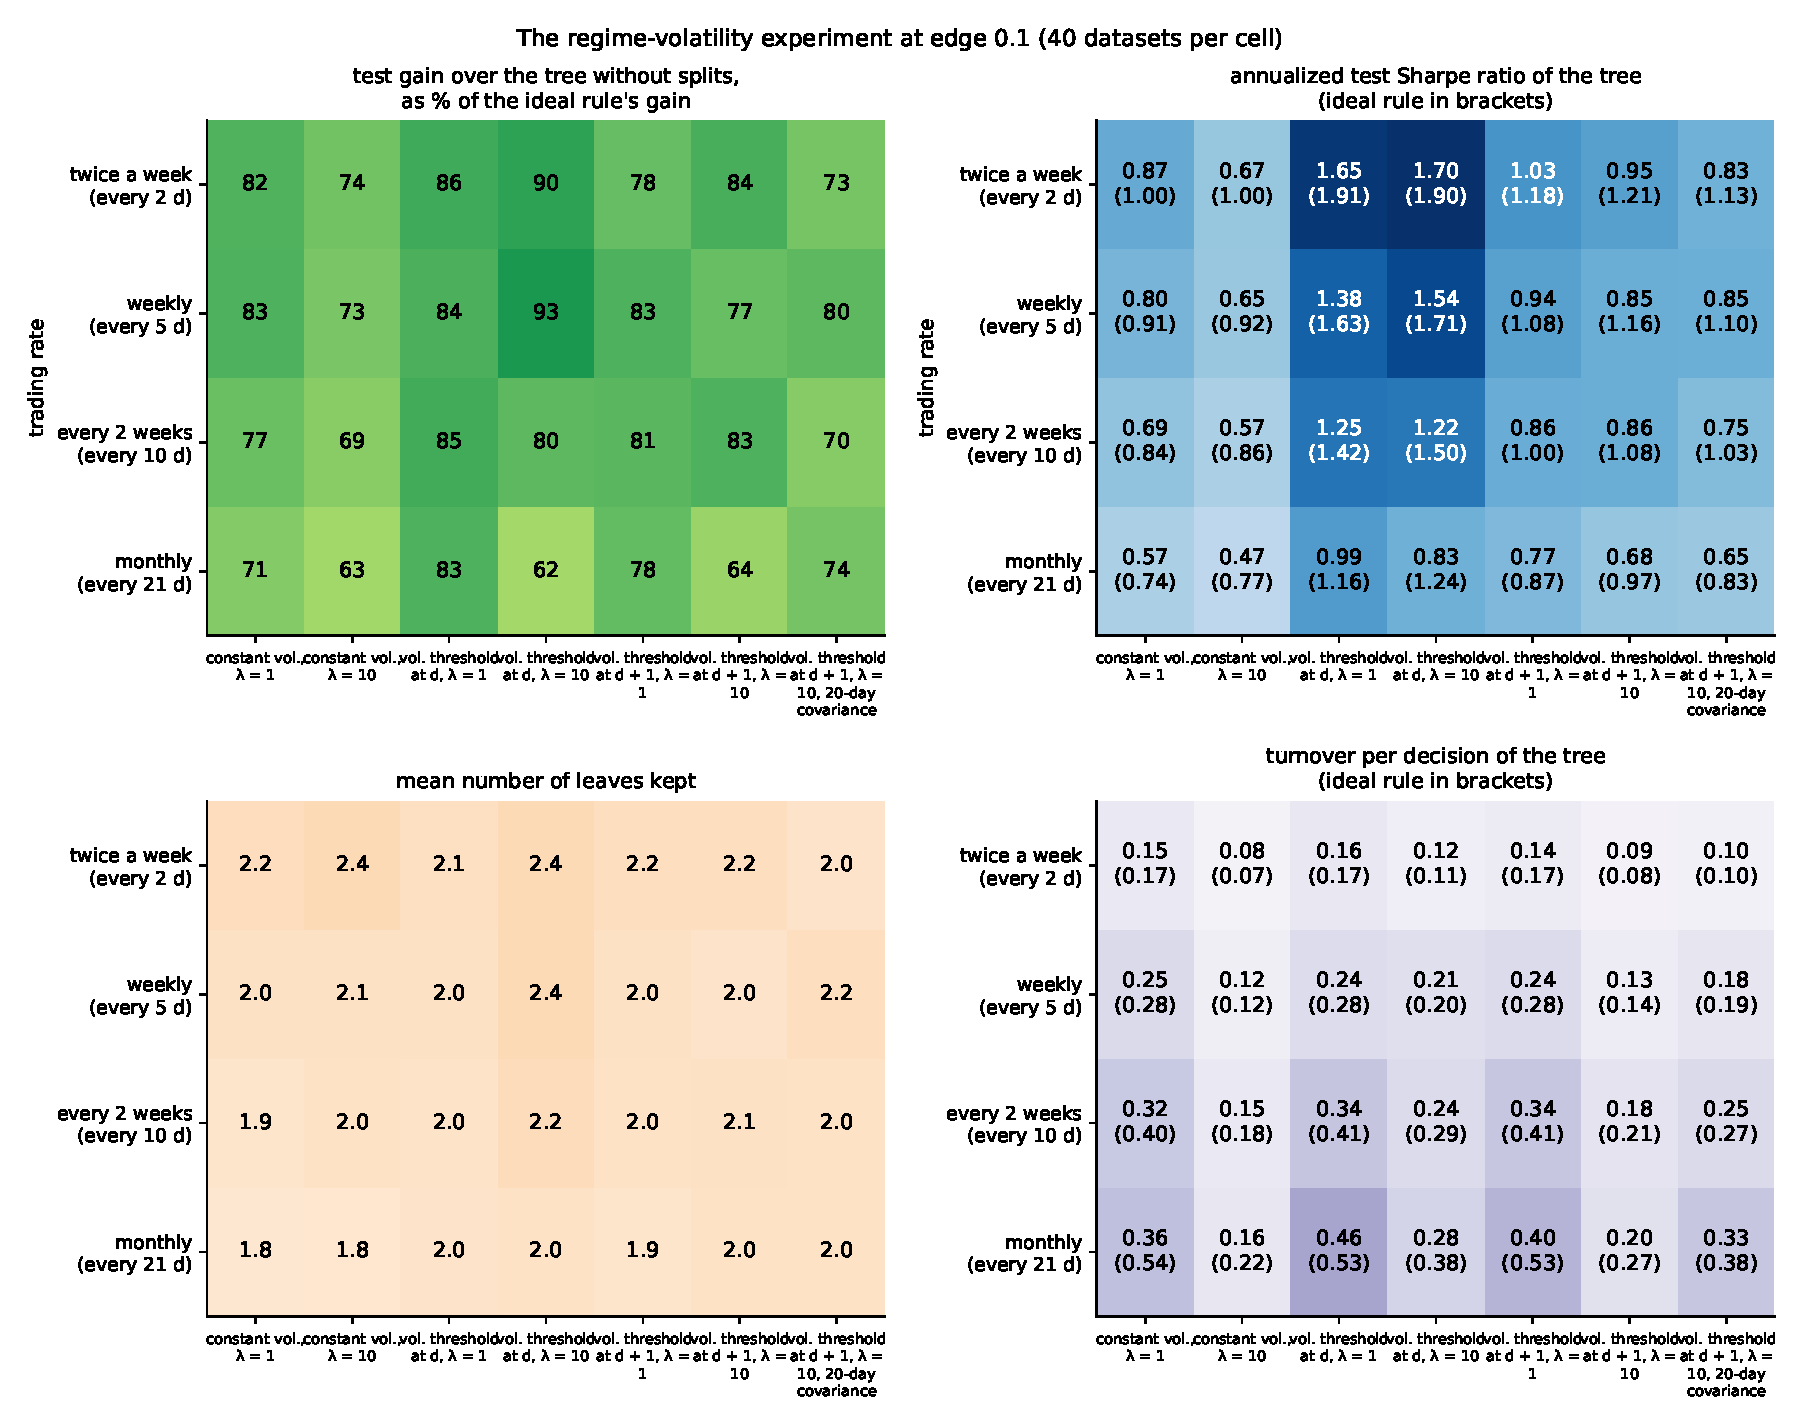
\includegraphics[width=0.95\linewidth]{regime_volatility_maps}
\caption{Edge 0.10, rows: trading rate, columns: setting. Share of the ideal rule's test gain captured; annualized test Sharpe ratio (ideal rule in brackets); mean number of leaves; turnover per decision (ideal rule in brackets).}
\label{fig:maps}
\end{figure}
\begin{figure}[H]
\centering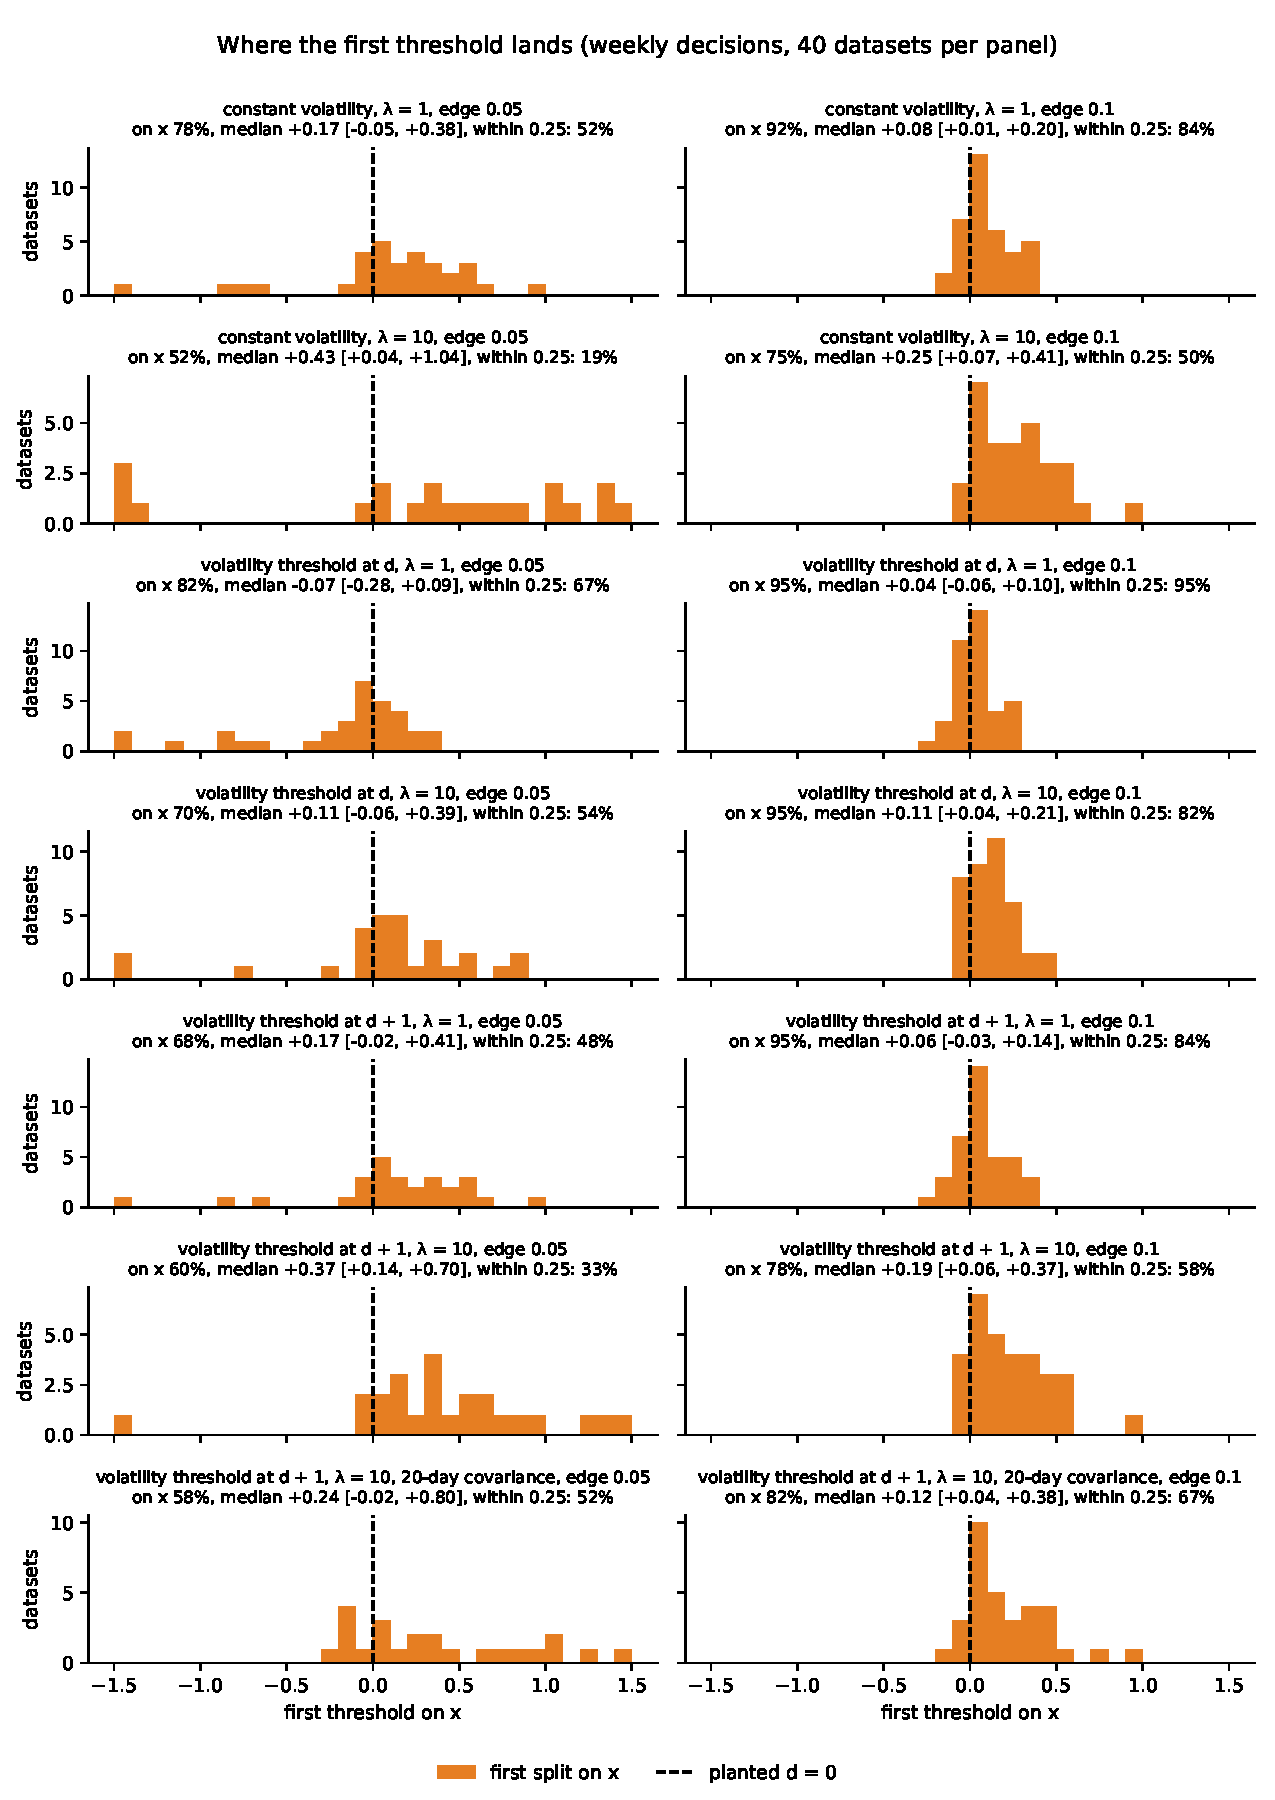
\includegraphics[width=0.9\linewidth]{regime_volatility_thresholds}
\caption{Weekly decisions: where the first threshold lands, one row per setting; \emph{left:} edge 0.05, \emph{right:} edge 0.10. The target is $d=0$.}
\label{fig:thresholds}
\end{figure}

\begin{table}[H]
\centering\scriptsize
\setlength{\tabcolsep}{2.4pt}
\begin{tabular}{@{}l r rr r rrr r rrr rrr@{}}
\toprule
& & \multicolumn{2}{c}{threshold} & near & \multicolumn{3}{c}{annualized test Sharpe} & gain & \multicolumn{3}{c}{position, $0<x<1$} & \multicolumn{3}{c}{position, $x>1$}\\
\cmidrule(lr){3-4}\cmidrule(lr){6-8}\cmidrule(lr){10-12}\cmidrule(lr){13-15}
setting & $h$ & on $x$ & $\le0.25$ & $d_\sigma$ & tree & ideal & true var. & capt. & tree & ideal & true var. & tree & ideal & true var.\\
\midrule
constant vol., $\lambda=1$ & 2 & 98 & 97 & -- & 0.87 & 1.00 & 1.00 & 82\% & 0.81 & 0.91 & 0.91 & 0.94 & 1.00 & 1.00\\
 & 5 & 92 & 84 & -- & 0.80 & 0.91 & 0.91 & 83\% & 0.79 & 0.90 & 0.90 & 0.95 & 1.00 & 1.00\\
 & 10 & 88 & 63 & -- & 0.69 & 0.84 & 0.83 & 77\% & 0.76 & 0.88 & 0.88 & 0.94 & 1.00 & 1.00\\
 & 21 & 72 & 45 & -- & 0.57 & 0.74 & 0.74 & 71\% & 0.65 & 0.87 & 0.87 & 0.84 & 1.00 & 1.00\\
\midrule
constant vol., $\lambda=10$ & 2 & 78 & 68 & -- & 0.67 & 1.00 & 1.01 & 74\% & 0.30 & 0.37 & 0.37 & 0.38 & 0.46 & 0.44\\
 & 5 & 75 & 50 & -- & 0.65 & 0.92 & 0.93 & 73\% & 0.27 & 0.34 & 0.34 & 0.42 & 0.49 & 0.48\\
 & 10 & 72 & 45 & -- & 0.57 & 0.86 & 0.87 & 69\% & 0.23 & 0.29 & 0.29 & 0.40 & 0.48 & 0.49\\
 & 21 & 68 & 11 & -- & 0.47 & 0.77 & 0.77 & 63\% & 0.15 & 0.23 & 0.23 & 0.37 & 0.45 & 0.45\\
\midrule
vol.\ threshold at $d$, $\lambda=1$ & 2 & 98 & 95 & 8 & 1.65 & 1.91 & 1.91 & 86\% & 0.80 & 0.91 & 0.91 & 0.89 & 1.00 & 1.00\\
 & 5 & 95 & 95 & 5 & 1.38 & 1.63 & 1.63 & 84\% & 0.87 & 0.91 & 0.90 & 0.99 & 1.00 & 1.00\\
 & 10 & 88 & 77 & 10 & 1.25 & 1.42 & 1.42 & 85\% & 0.83 & 0.89 & 0.90 & 0.98 & 1.00 & 1.00\\
 & 21 & 88 & 69 & 5 & 0.99 & 1.16 & 1.13 & 83\% & 0.83 & 0.89 & 0.91 & 0.98 & 1.00 & 1.00\\
\midrule
vol.\ threshold at $d$, $\lambda=10$ & 2 & 98 & 95 & 20 & 1.70 & 1.90 & 1.93 & 90\% & 0.60 & 0.65 & 0.90 & 0.79 & 0.83 & 1.00\\
 & 5 & 95 & 82 & 12 & 1.54 & 1.71 & 1.70 & 93\% & 0.59 & 0.60 & 0.85 & 0.83 & 0.87 & 1.00\\
 & 10 & 82 & 64 & 12 & 1.22 & 1.50 & 1.50 & 80\% & 0.47 & 0.53 & 0.80 & 0.77 & 0.88 & 1.00\\
 & 21 & 72 & 38 & 10 & 0.83 & 1.24 & 1.22 & 62\% & 0.34 & 0.44 & 0.74 & 0.65 & 0.85 & 1.00\\
\midrule
vol.\ threshold at $d+1$, $\lambda=1$ & 2 & 95 & 97 & 0 & 1.03 & 1.18 & 1.18 & 78\% & 0.79 & 0.91 & 0.91 & 0.94 & 1.00 & 1.00\\
 & 5 & 95 & 84 & 0 & 0.94 & 1.08 & 1.08 & 83\% & 0.82 & 0.90 & 0.90 & 0.99 & 1.00 & 1.00\\
 & 10 & 90 & 58 & 0 & 0.86 & 1.00 & 1.00 & 81\% & 0.79 & 0.89 & 0.88 & 0.98 & 1.00 & 1.00\\
 & 21 & 80 & 53 & 5 & 0.77 & 0.87 & 0.87 & 78\% & 0.70 & 0.88 & 0.87 & 0.90 & 1.00 & 1.00\\
\midrule
vol.\ threshold at $d+1$, $\lambda=10$ & 2 & 85 & 85 & 10 & 0.95 & 1.21 & 1.34 & 84\% & 0.38 & 0.45 & 0.40 & 0.52 & 0.58 & 0.96\\
 & 5 & 78 & 58 & 8 & 0.85 & 1.16 & 1.23 & 77\% & 0.33 & 0.41 & 0.35 & 0.53 & 0.63 & 0.95\\
 & 10 & 80 & 53 & 5 & 0.86 & 1.08 & 1.12 & 83\% & 0.31 & 0.35 & 0.29 & 0.57 & 0.64 & 0.93\\
 & 21 & 70 & 11 & 12 & 0.68 & 0.97 & 0.94 & 64\% & 0.19 & 0.28 & 0.23 & 0.47 & 0.60 & 0.91\\
\midrule
same, 20-day covariance & 2 & 78 & 81 & 2 & 0.83 & 1.13 & 1.28 & 73\% & 0.40 & 0.50 & 0.40 & 0.69 & 0.85 & 0.96\\
 & 5 & 82 & 67 & 8 & 0.85 & 1.10 & 1.21 & 80\% & 0.40 & 0.44 & 0.35 & 0.75 & 0.85 & 0.95\\
 & 10 & 75 & 73 & 8 & 0.75 & 1.03 & 1.13 & 70\% & 0.34 & 0.38 & 0.29 & 0.69 & 0.84 & 0.93\\
 & 21 & 72 & 34 & 8 & 0.65 & 0.83 & 0.85 & 74\% & 0.25 & 0.29 & 0.22 & 0.62 & 0.78 & 0.90\\
\bottomrule
\end{tabular}
\caption{Edge 0.10, 40 datasets per row ($h$: days between decisions). ``on $x$'' and ``$\le0.25$'': share of datasets whose first split is on $x$, and whose first threshold is within $0.25$ of $d$; ``near $d_\sigma$'': share with a second-level split within $0.25$ of the volatility threshold; ``true var.'': the ideal rule with the regime's own variance; ``capt.'': share of the ideal rule's gain captured; positions: mean weight of the asset on the test decisions with $0<x<1$ (the stressed part of the good regime when $d_\sigma=1$) and with $x>1$ (the calm part). At edge 0.05 the volatility threshold at $d$ doubles the tree's Sharpe ratio too (0.46--0.51 against 0.19--0.27) and the tree captures 47--70\% of the gain; the other settings behave as at edge 0.10 with every number smaller.}
\label{tab:regime}
\end{table}

\textbf{Reading the figures and the table.}
\begin{itemize}\setlength{\itemsep}{1pt}
\item \textbf{Asymmetric noise helps the drift threshold.} With the volatility threshold at $d$ the good regime has half the noise, and the threshold is found more often (88\% monthly against 72\%) and more precisely (95\% within $0.25$ at weekly decisions against 84\%); the tree captures 83 to 86\% of the ideal gain against 71 to 83\%. The Sharpe ratios of every rule roughly double, because the money is made in the calm regime.
\item \textbf{At $\lambda=10$ the tree sizes its positions as the ideal rule on the same information does} (0.60 against 0.65 in the stressed band, 0.79 against 0.83 in the calm one when $d_\sigma=d$), and captures 80 to 93\% of the gain at the fast rates; it loses ground monthly (62\%), as in the planted-threshold report.
\item \textbf{The volatility boundary at $d+1$ is not learnt.} At $\lambda=10$ the clairvoyant rule holds 0.96 of the asset in the calm regime and 0.40 in the stressed one; the tree holds 0.52 and 0.38, the ideal rule on the same information 0.58 and 0.45. Second-level splits land near $x=1$ in 5 to 12\% of the datasets only (Figure~\ref{fig:splits}), no more than with constant volatility. The tree's regret is computed with the covariance estimate of the last 180 days, the same one the optimizer uses; that estimate averages over regimes, so in the loss the calm regime is not less risky than the stressed one and a split at $d_\sigma$ has nothing to gain. The tree cannot learn what its own utility does not reward.
\item \textbf{A 20-day covariance window lets the estimate follow the regime but pays for its noise.} The tree's calm-regime position rises to 0.69--0.75, yet its Sharpe ratio does not improve (0.83 against 0.95 at every 2 days), and the ideal rule on the same information falls from 1.16 to 1.10 at weekly decisions: the estimate's noise costs more than the regime tracking gains.
\item \textbf{What the true variance is worth}: about 0.1 of annual Sharpe at the fast rates when the volatility boundary sits inside the good regime (1.23 against 1.16 at weekly decisions), nothing when it coincides with the drift threshold, since sizing a regime whose Sharpe ratio is constant does not change its Sharpe ratio.
\end{itemize}

\section{What this says}\label{sec:says}
\begin{itemize}\setlength{\itemsep}{1pt}
\item A regime feature that also drives the volatility is easier, not harder, for the tree, as long as the calm regime is the profitable one: the decision threshold is pinned by the clean returns.
\item A volatility regime enters the pipeline only through the covariance the optimizer and the regret use. To exploit a volatility boundary, the pipeline needs a covariance estimate that responds to the regime (a variance forecast from the feature itself, or an exponentially weighted estimate with a short half-life) rather than a longer or deeper tree; with a lagged estimate the tree correctly does not split on it.
\item The next test is therefore on the risk model, not on the tree: give the optimizer a variance that knows the regime and check that the second split appears at $d_\sigma$.
\end{itemize}

\section{How to reproduce}
\begin{itemize}\raggedright\setlength{\itemsep}{1pt}
\item \code{python planted_threshold_experiments.py} \code{run-regime}: the seven settings, 2{,}240 fits; writes \code{results_regime_volatility.json} in \code{report/figures/}.
\item \code{python planted_threshold_experiments.py} \code{plot}: the figures \code{regime_volatility_*} and the summary table.
\item The model is \code{synthetic_market.signal_process} with \code{up_volatility_ratio=0.5} and \code{volatility_threshold}; the settings are fields of \code{Case} in \code{planted_threshold_test.py}; the tree and its options are described in \code{model_and_training_pipeline.tex}.
\end{itemize}
\end{document}
